% Include with % Include with % Include with % Include with \input{chance-dp}; keep the figures/ subdirectory alongside the main
% manuscript or add their directory to \graphicspath. Requires amsmath,
% amssymb, and graphicx.
\subsection{The standard dynamic programming model}
We consider a portfolio with initial wealth $W_0=\$100$ million and a nominal terminal floor $F=\$95$ million. At each trading session $t$, the investor observes wealth $W_t$ and a volatility regime $z_t$, and allocates a fraction $a_t\in\mathcal A_0=\{0,0.25,0.50,0.75,1\}$ to equity. The balance earns the daily cash rate $r_f=0.02/252$. If $X_{t+1}$ denotes the equity return in excess of cash, wealth evolves as $W_{t+1}=W_t(1+r_f+a_tX_{t+1})$.

The high-volatility regime applies when the pre-trade volatility forecast exceeds its historical 80th percentile. In the planning model, the two equally likely excess returns are $\mu\pm\sigma_z/\sqrt{252}$, where $\mu=0.05/252$ and annual volatility is $0.15$ in the ordinary regime and $0.30$ in the high regime. The regime switches independently of the return shock, with daily transition probabilities of $0.01$ from ordinary to high and $0.04$ from high to ordinary.

The investor values terminal wealth through $u(x)=-1/x-5(0.95-x)^+$, where $x=W_T/W_0$ and $y^+=\max(y,0)$. The second term penalizes the magnitude of a terminal shortfall. Starting from $V_T(w,z)=u(w/W_0)$, backward induction gives
\begin{equation}
 V_t(w,z)=\max_{a\in\mathcal A_0}
 \mathbb E\!\left[V_{t+1}\bigl(w(1+r_f+aX_{t+1}),z_{t+1}\bigr)\mid z_t=z\right].
\end{equation}

\subsection{Chance-constrained dynamic programming}
We extend the baseline model to pursue higher mean terminal wealth while keeping the modeled probability of finishing below the floor under 2\%.
\paragraph{Wealth-dependent equity cap.}
The baseline model allows full equity exposure even when wealth is just above the floor. We cap equity exposure according to the dollar cushion $C(w)=(w-F)^+$. The cap allows $m$ dollars of equity exposure per dollar of cushion up to $K=\$5$ million, and $1.5m$ dollars per additional dollar of cushion. Total equity exposure is bounded by
\begin{equation}
 E_{\max}(w)=\min\!\left\{w,\;m\min(C(w),K)+1.5m\bigl(C(w)-K\bigr)^+\right\}.
\end{equation}
The admissible dollar positions comprise the baseline positions $aw$, $a\in\mathcal A_0$, clipped to $E_{\max}(w)$, together with 25\%, 50\%, and 75\% of the cap. These intermediate positions preserve allocation choices near the floor, where several baseline positions collapse to the same cap. At or below the floor, the portfolio holds cash. Each launch retains the multiplier selected for its opening year using only previously completed investments.

\paragraph{Rare downside shocks.}
A sharp one-day loss can exhaust the cushion even when the equity position satisfies the cap. To capture this risk, we add a rare downside shock to each regime. The model assigns a daily probability $p_z$ to an excess return $g_z$, with $(p_z,g_z)=(0.001,-0.10)$ in the ordinary regime and $(0.004,-0.20)$ in the high regime. The remaining two outcomes, $c_z\pm\sigma_z/\sqrt{252}$, each receive probability $(1-p_z)/2$. Choosing $c_z=(\mu-p_zg_z)/(1-p_z)$ preserves the baseline expected equity premium.

\paragraph{Terminal probability constraint.}
The baseline utility penalizes the size of a shortfall but places no limit on its probability. We impose that limit directly and maximize expected terminal wealth subject to it. For the launch state $s_0=(W_0,z_0)$ and the prescribed maturity $T$, the target problem is
\begin{equation}
 \max_{\pi}\;\mathbb E_{\pi}[W_T\mid s_0]
 \quad\text{subject to}\quad
 \Pr_{\pi}(W_T<F\mid s_0)<0.02 .
\end{equation}
We approximate this problem with four candidate policies and an all-cash alternative. For each breach penalty $\lambda\in\{0,10,100,1000\}$ million dollars, backward induction uses the terminal payoff $W_T-\lambda\mathbf{1}_{\{W_T<F\}}$ and tracks both expected terminal wealth and breach probability under the resulting policy. At launch, the strategy selects the candidate with the highest modeled mean among those satisfying the probability limit. The selected policy remains fixed through maturity, while its equity allocation responds daily to wealth, regime, and time remaining.

Figures~\ref{fig:ccdp-vol} and~\ref{fig:ccdp-cdf} show the allocation rules and historical terminal wealth distributions for the four cumulative specifications. The first three maximize the original terminal utility, which isolates the effect of changing the action set and then the transition law. The fourth introduces the constrained mean-wealth objective. All four use realized equity and cash returns in the historical replay. Across 910 launches, the equity cap reduces the number of terminal breaches from 34 to one. Each subsequent specification also records one breach. Under the gap model, replacing terminal utility with the constrained mean-wealth objective raises historical mean terminal wealth from \$109.11 million to \$109.85 million.

\begin{figure*}[tbp]
 \centering
 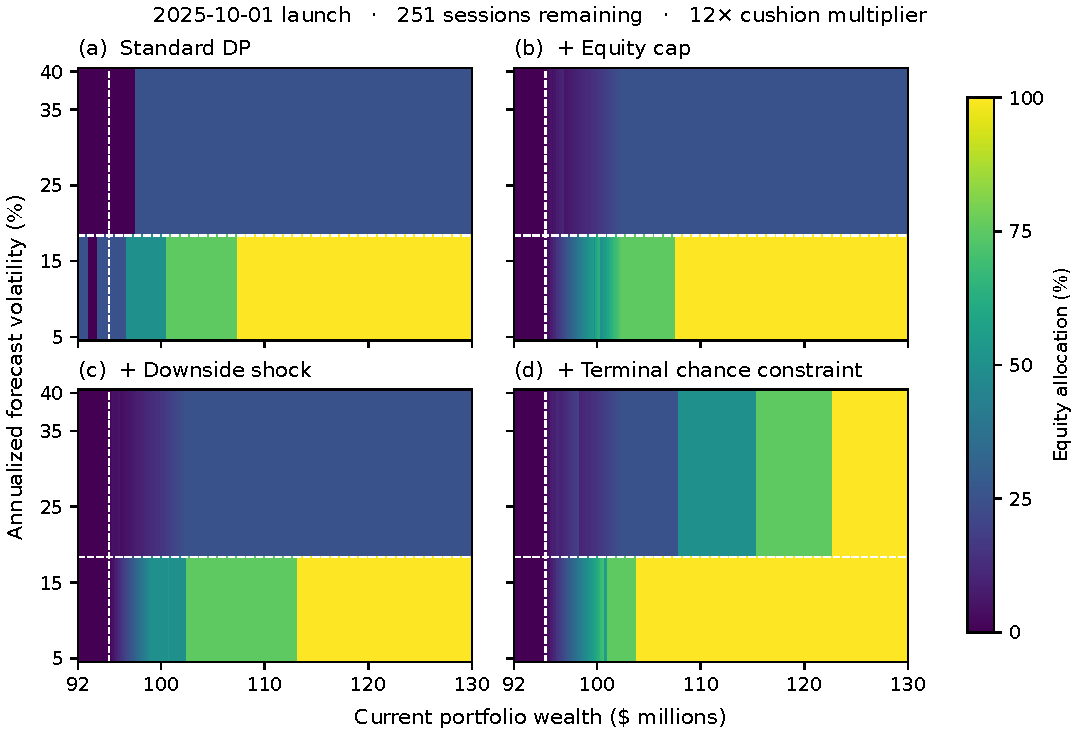
\includegraphics[width=0.93\textwidth]{figures/wealth-volatility.pdf}
 \caption{Equity allocation as a function of current wealth and forecast volatility for the latest eligible 12-month launch. Each panel quotes a strategy at the same remaining horizon. Color gives the percentage of wealth invested in equity. The vertical dashed line marks the \$95 million floor and the horizontal dashed line marks the launch volatility cutoff. Panel (d) retains the policy selected at launch across all plotted states.}
 \label{fig:ccdp-vol}
\end{figure*}

\begin{figure*}[tbp]
 \centering
 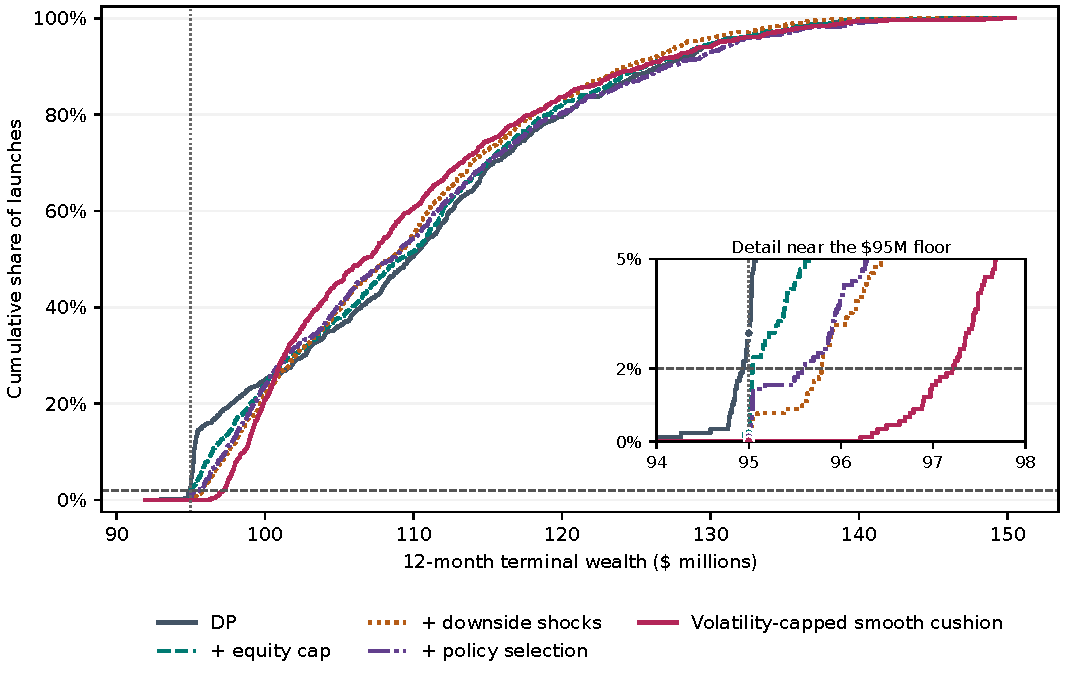
\includegraphics[width=0.87\textwidth]{figures/terminal-cdf.pdf}
 \caption{Empirical cumulative distributions of terminal wealth for 910 overlapping 12-month investments launched monthly from January 1950 through October 2025. At each wealth level, the curve gives the fraction of launches ending at or below that level. The inset spans \$94--96 million and cumulative probabilities from 0 to 5\%. Dots mark the empirical CDF at \$95 million. The three capped strategies coincide there. Horizontal dashed lines mark 2\%. The left limit at the \$95 million floor gives the historical terminal breach rate. The 2\% policy limit applies to the modeled probability at launch.}
 \label{fig:ccdp-cdf}
\end{figure*}


\subsection{Smooth Variant}
The chance-constrained DP heatmap suggests a simpler daily rule. Moving right in Figure~\ref{fig:ccdp-vol}(d), a larger cushion supports more equity. Moving upward, even a small change in forecast volatility can switch the regime and abruptly change the position. The smooth variant preserves the cushion response and uses the volatility forecast directly to reduce exposure gradually.

\paragraph{Why discount the floor?}
At \$100 million of wealth and 15\% forecast volatility, the October 2025 DP policy allocates 60\% to equity with 251 sessions left and 50\% with one session left. The smooth rule captures this horizon effect through the cost of funding the floor. At the modeled cash rate, the reserve needed to fund \$95 million at maturity rises from \$93.13 million to \$94.99 million between those dates. At the same wealth, this leaves \$6.87 million of cushion early in the year and only \$5.01 million on the final trading day.

\paragraph{Daily allocation.}
Measure wealth in millions of dollars. With $n=T-t$ sessions remaining, the reserve is $F_n=F(1+r_f)^{-n}$ and the cushion is $c=(W_t-F_n)^+$. Define base equity exposure by $G(c)=\int_0^c h(u)\,du$, where
\[
 h(u)=1+\frac{(u-3)^+-(u-7)^+}{2}
       +\frac{(u-15)^+-(u-25)^+}{10}.
\]
Each additional cushion dollar initially supports one dollar of base equity exposure. Its contribution rises gradually to three dollars over the \$3--7 million band and to four over the \$15--25 million band.

For annualized forecast volatility $v$ and launch scale $s$, the rule reduces the requested equity fraction $r$ as volatility rises and sets a ceiling $L(v)$ according to
\[
 r=1.25\,s\,\frac{3}{[1+(v/0.10)^6]^{1/6}}\frac{G(c)}{W_t},
 \qquad L(v)=\frac{1}{1+(v/0.30)^4}.
\]
Each session the strategy rebalances to equity holdings of $a_t W_t$, where the target fraction is
\[
 a_t=\frac{r}{[1+(r/L(v))^4]^{1/4}}.
\]
Near the reserve, the rule grants approximately the requested fraction. With ample cushion, the weight approaches the volatility ceiling, which falls from 50\% at 30\% volatility to 24\% at 40\% volatility (Figure~\ref{fig:smooth-vol}). The breakpoints and ceiling are design choices motivated by the DP surface. Each one-year launch inherits the scale selected on completed launches for the earlier time-aware cushion rule. During sparse-history warm-up it uses unit scale and the nominal floor.

Table~\ref{tab:strategy-overview} compares all five strategies on the same 12-month launches. Table~\ref{tab:strategy-comparison} then compares the final two strategies on the committee's objective and floor. The chance-constrained DP achieved higher overall certainty-equivalent wealth at both horizons, while the smooth rule achieved higher certainty-equivalent wealth on crisis launches at both horizons. Of these two strategies, only the DP breached the floor, on one lower-volatility 12-month launch. Over all 12-month launches, the worst finish was \$94.996 million for the DP and \$95.230 million for the smooth rule. Figure~\ref{fig:smooth-cdf} shows the crossing distributions near the floor.

\begin{table*}[tbp]
 \centering
 \caption{Certainty-equivalent wealth, mean terminal wealth, and floor breaches for 910 overlapping 12-month investments of \$100 million each, launched monthly from January 1950 through October 2025. A launch is classified as crisis if the equity total-return index closed at least 20\% below its trailing 12-month high on the previous trading day. For all other launches, higher volatility means that the volatility of daily equity returns over the preceding 63 trading sessions exceeded the median across all earlier 63-session windows. Lower volatility includes values at or below that median.}
 \label{tab:strategy-overview}
 \small
 \input{figures/strategy-overview.tex}
 \par\smallskip
 \begin{minipage}{0.96\linewidth}\footnotesize
 For each launch group, the objective value at $\gamma=2$ is $\mathrm{CE}=(n^{-1}\sum_{i=1}^{n}1/W_{T,i})^{-1}$. Breaches count finishes strictly below \$95 million. Percentages use the same group. Within each group, bold marks the highest CE among strategies with observed breach rates at or below 2\% in every launch condition, the highest arithmetic mean, and the fewest breaches (including ties).
 \end{minipage}
\end{table*}

\begin{table*}[tbp]
 \centering
 \caption{Historical certainty-equivalent terminal wealth and floor breaches from a \$100 million investment, by market condition at launch.}
 \label{tab:strategy-comparison}
 \small
 \input{figures/strategy-comparison.tex}
 \par\smallskip
 \begin{minipage}{0.96\linewidth}\footnotesize
 CE is the harmonic mean of terminal wealth ($\gamma=2$). Breaches count launches finishing strictly below \$95 million, with the observed rate in parentheses. Monthly launches overlap, so these rates alone cannot establish a 2\% upper bound on breach probability. The smooth rule uses its historically selected scale at 12 months and a fixed scale of one at 24 months.
 \end{minipage}
\end{table*}

\begin{figure*}[tbp]
 \centering
 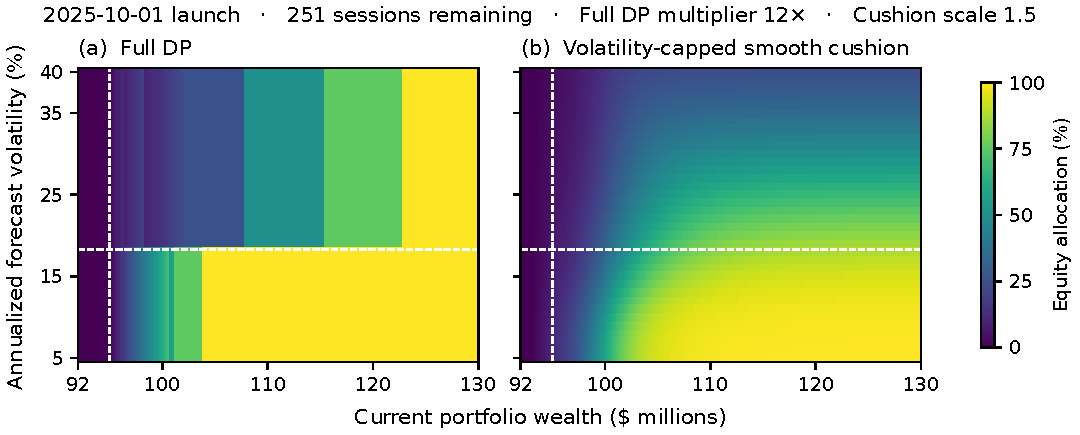
\includegraphics[width=0.93\textwidth]{figures/smooth-wealth-volatility.pdf}
 \caption{Equity weights for the same October 2025 launch and wealth--volatility grid as Figure~\ref{fig:ccdp-vol}. The vertical line marks the nominal terminal floor. The horizontal line marks the DP regime cutoff, shown on both panels for reference. Both policies retain their launch settings.}
 \label{fig:smooth-vol}
\end{figure*}

\begin{figure*}[tbp]
 \centering
 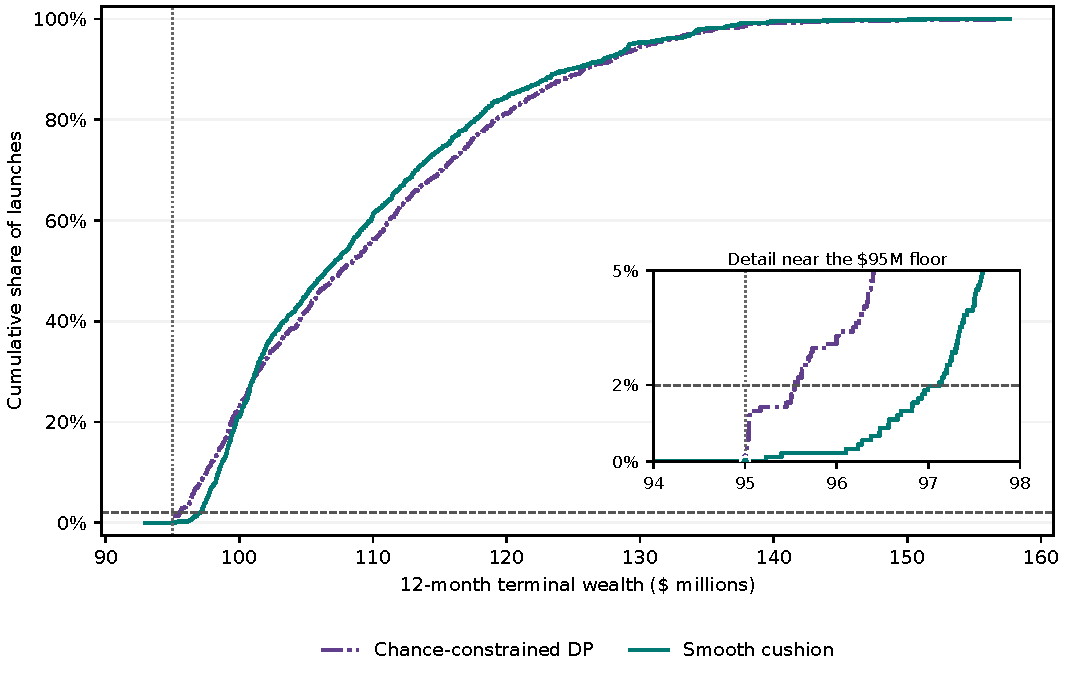
\includegraphics[width=0.87\textwidth]{figures/smooth-terminal-cdf.pdf}
 \caption{Terminal wealth for the chance-constrained DP and smooth cushion on the same 910 monthly launches as Figure~\ref{fig:ccdp-cdf}. The inset shows the share finishing at or below each wealth level from \$94 to \$98 million. Dots mark the share at \$95 million and the horizontal dashed line marks 2\%.}
 \label{fig:smooth-cdf}
\end{figure*}
; keep the figures/ subdirectory alongside the main
% manuscript or add their directory to \graphicspath. Requires amsmath,
% amssymb, and graphicx.
\subsection{The standard dynamic programming model}
We consider a portfolio with initial wealth $W_0=\$100$ million and a nominal terminal floor $F=\$95$ million. At each trading session $t$, the investor observes wealth $W_t$ and a volatility regime $z_t$, and allocates a fraction $a_t\in\mathcal A_0=\{0,0.25,0.50,0.75,1\}$ to equity. The balance earns the daily cash rate $r_f=0.02/252$. If $X_{t+1}$ denotes the equity return in excess of cash, wealth evolves as $W_{t+1}=W_t(1+r_f+a_tX_{t+1})$.

The high-volatility regime applies when the pre-trade volatility forecast exceeds its historical 80th percentile. In the planning model, the two equally likely excess returns are $\mu\pm\sigma_z/\sqrt{252}$, where $\mu=0.05/252$ and annual volatility is $0.15$ in the ordinary regime and $0.30$ in the high regime. The regime switches independently of the return shock, with daily transition probabilities of $0.01$ from ordinary to high and $0.04$ from high to ordinary.

The investor values terminal wealth through $u(x)=-1/x-5(0.95-x)^+$, where $x=W_T/W_0$ and $y^+=\max(y,0)$. The second term penalizes the magnitude of a terminal shortfall. Starting from $V_T(w,z)=u(w/W_0)$, backward induction gives
\begin{equation}
 V_t(w,z)=\max_{a\in\mathcal A_0}
 \mathbb E\!\left[V_{t+1}\bigl(w(1+r_f+aX_{t+1}),z_{t+1}\bigr)\mid z_t=z\right].
\end{equation}

\subsection{Chance-constrained dynamic programming}
We extend the baseline model to pursue higher mean terminal wealth while keeping the modeled probability of finishing below the floor under 2\%.
\paragraph{Wealth-dependent equity cap.}
The baseline model allows full equity exposure even when wealth is just above the floor. We cap equity exposure according to the dollar cushion $C(w)=(w-F)^+$. The cap allows $m$ dollars of equity exposure per dollar of cushion up to $K=\$5$ million, and $1.5m$ dollars per additional dollar of cushion. Total equity exposure is bounded by
\begin{equation}
 E_{\max}(w)=\min\!\left\{w,\;m\min(C(w),K)+1.5m\bigl(C(w)-K\bigr)^+\right\}.
\end{equation}
The admissible dollar positions comprise the baseline positions $aw$, $a\in\mathcal A_0$, clipped to $E_{\max}(w)$, together with 25\%, 50\%, and 75\% of the cap. These intermediate positions preserve allocation choices near the floor, where several baseline positions collapse to the same cap. At or below the floor, the portfolio holds cash. Each launch retains the multiplier selected for its opening year using only previously completed investments.

\paragraph{Rare downside shocks.}
A sharp one-day loss can exhaust the cushion even when the equity position satisfies the cap. To capture this risk, we add a rare downside shock to each regime. The model assigns a daily probability $p_z$ to an excess return $g_z$, with $(p_z,g_z)=(0.001,-0.10)$ in the ordinary regime and $(0.004,-0.20)$ in the high regime. The remaining two outcomes, $c_z\pm\sigma_z/\sqrt{252}$, each receive probability $(1-p_z)/2$. Choosing $c_z=(\mu-p_zg_z)/(1-p_z)$ preserves the baseline expected equity premium.

\paragraph{Terminal probability constraint.}
The baseline utility penalizes the size of a shortfall but places no limit on its probability. We impose that limit directly and maximize expected terminal wealth subject to it. For the launch state $s_0=(W_0,z_0)$ and the prescribed maturity $T$, the target problem is
\begin{equation}
 \max_{\pi}\;\mathbb E_{\pi}[W_T\mid s_0]
 \quad\text{subject to}\quad
 \Pr_{\pi}(W_T<F\mid s_0)<0.02 .
\end{equation}
We approximate this problem with four candidate policies and an all-cash alternative. For each breach penalty $\lambda\in\{0,10,100,1000\}$ million dollars, backward induction uses the terminal payoff $W_T-\lambda\mathbf{1}_{\{W_T<F\}}$ and tracks both expected terminal wealth and breach probability under the resulting policy. At launch, the strategy selects the candidate with the highest modeled mean among those satisfying the probability limit. The selected policy remains fixed through maturity, while its equity allocation responds daily to wealth, regime, and time remaining.

Figures~\ref{fig:ccdp-vol} and~\ref{fig:ccdp-cdf} show the allocation rules and historical terminal wealth distributions for the four cumulative specifications. The first three maximize the original terminal utility, which isolates the effect of changing the action set and then the transition law. The fourth introduces the constrained mean-wealth objective. All four use realized equity and cash returns in the historical replay. Across 910 launches, the equity cap reduces the number of terminal breaches from 34 to one. Each subsequent specification also records one breach. Under the gap model, replacing terminal utility with the constrained mean-wealth objective raises historical mean terminal wealth from \$109.11 million to \$109.85 million.

\begin{figure*}[tbp]
 \centering
 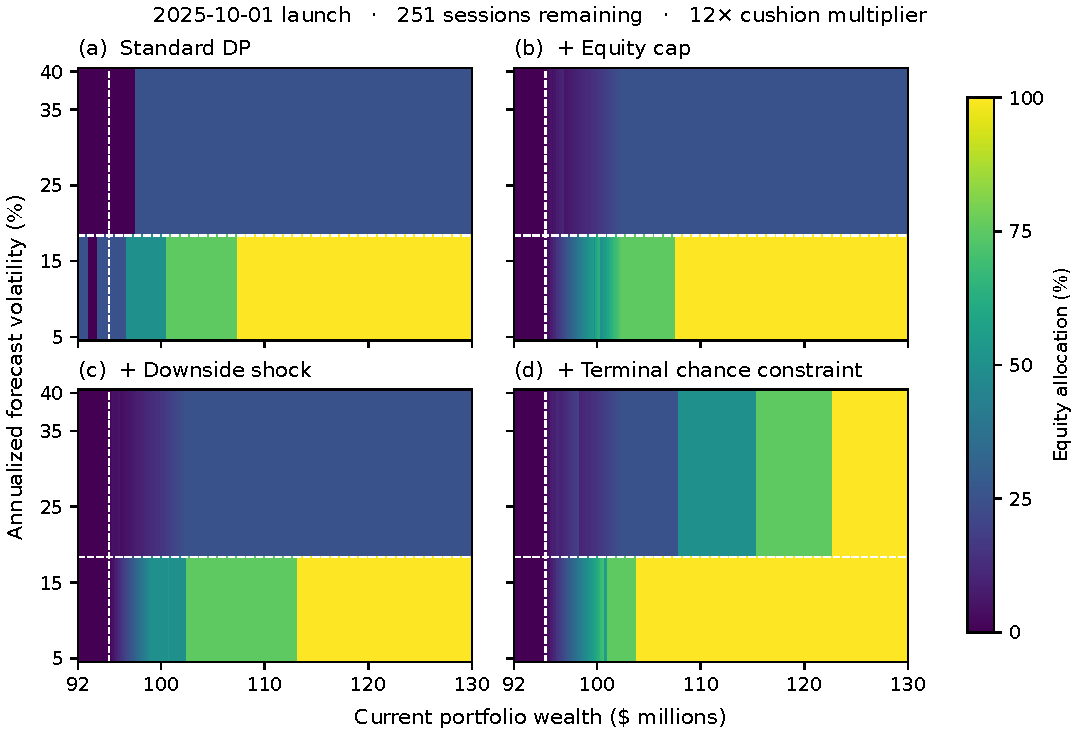
\includegraphics[width=0.93\textwidth]{figures/wealth-volatility.pdf}
 \caption{Equity allocation as a function of current wealth and forecast volatility for the latest eligible 12-month launch. Each panel quotes a strategy at the same remaining horizon. Color gives the percentage of wealth invested in equity. The vertical dashed line marks the \$95 million floor and the horizontal dashed line marks the launch volatility cutoff. Panel (d) retains the policy selected at launch across all plotted states.}
 \label{fig:ccdp-vol}
\end{figure*}

\begin{figure*}[tbp]
 \centering
 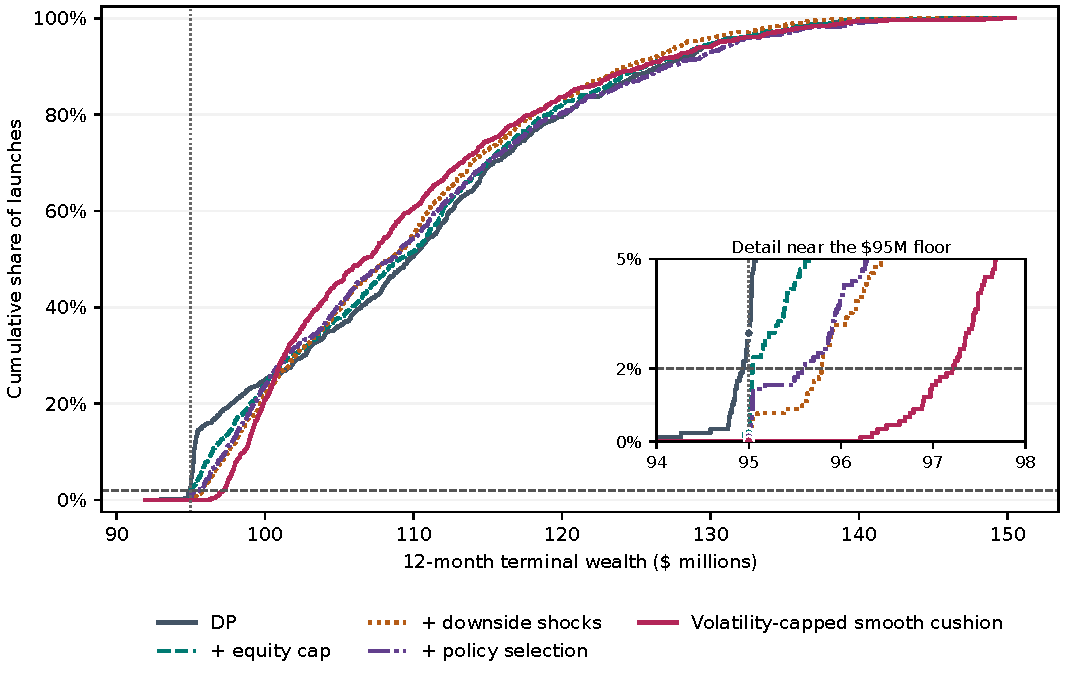
\includegraphics[width=0.87\textwidth]{figures/terminal-cdf.pdf}
 \caption{Empirical cumulative distributions of terminal wealth for 910 overlapping 12-month investments launched monthly from January 1950 through October 2025. At each wealth level, the curve gives the fraction of launches ending at or below that level. The inset spans \$94--96 million and cumulative probabilities from 0 to 5\%. Dots mark the empirical CDF at \$95 million. The three capped strategies coincide there. Horizontal dashed lines mark 2\%. The left limit at the \$95 million floor gives the historical terminal breach rate. The 2\% policy limit applies to the modeled probability at launch.}
 \label{fig:ccdp-cdf}
\end{figure*}


\subsection{Smooth Variant}
The chance-constrained DP heatmap suggests a simpler daily rule. Moving right in Figure~\ref{fig:ccdp-vol}(d), a larger cushion supports more equity. Moving upward, even a small change in forecast volatility can switch the regime and abruptly change the position. The smooth variant preserves the cushion response and uses the volatility forecast directly to reduce exposure gradually.

\paragraph{Why discount the floor?}
At \$100 million of wealth and 15\% forecast volatility, the October 2025 DP policy allocates 60\% to equity with 251 sessions left and 50\% with one session left. The smooth rule captures this horizon effect through the cost of funding the floor. At the modeled cash rate, the reserve needed to fund \$95 million at maturity rises from \$93.13 million to \$94.99 million between those dates. At the same wealth, this leaves \$6.87 million of cushion early in the year and only \$5.01 million on the final trading day.

\paragraph{Daily allocation.}
Measure wealth in millions of dollars. With $n=T-t$ sessions remaining, the reserve is $F_n=F(1+r_f)^{-n}$ and the cushion is $c=(W_t-F_n)^+$. Define base equity exposure by $G(c)=\int_0^c h(u)\,du$, where
\[
 h(u)=1+\frac{(u-3)^+-(u-7)^+}{2}
       +\frac{(u-15)^+-(u-25)^+}{10}.
\]
Each additional cushion dollar initially supports one dollar of base equity exposure. Its contribution rises gradually to three dollars over the \$3--7 million band and to four over the \$15--25 million band.

For annualized forecast volatility $v$ and launch scale $s$, the rule reduces the requested equity fraction $r$ as volatility rises and sets a ceiling $L(v)$ according to
\[
 r=1.25\,s\,\frac{3}{[1+(v/0.10)^6]^{1/6}}\frac{G(c)}{W_t},
 \qquad L(v)=\frac{1}{1+(v/0.30)^4}.
\]
Each session the strategy rebalances to equity holdings of $a_t W_t$, where the target fraction is
\[
 a_t=\frac{r}{[1+(r/L(v))^4]^{1/4}}.
\]
Near the reserve, the rule grants approximately the requested fraction. With ample cushion, the weight approaches the volatility ceiling, which falls from 50\% at 30\% volatility to 24\% at 40\% volatility (Figure~\ref{fig:smooth-vol}). The breakpoints and ceiling are design choices motivated by the DP surface. Each one-year launch inherits the scale selected on completed launches for the earlier time-aware cushion rule. During sparse-history warm-up it uses unit scale and the nominal floor.

Table~\ref{tab:strategy-overview} compares all five strategies on the same 12-month launches. Table~\ref{tab:strategy-comparison} then compares the final two strategies on the committee's objective and floor. The chance-constrained DP achieved higher overall certainty-equivalent wealth at both horizons, while the smooth rule achieved higher certainty-equivalent wealth on crisis launches at both horizons. Of these two strategies, only the DP breached the floor, on one lower-volatility 12-month launch. Over all 12-month launches, the worst finish was \$94.996 million for the DP and \$95.230 million for the smooth rule. Figure~\ref{fig:smooth-cdf} shows the crossing distributions near the floor.

\begin{table*}[tbp]
 \centering
 \caption{Certainty-equivalent wealth, mean terminal wealth, and floor breaches for 910 overlapping 12-month investments of \$100 million each, launched monthly from January 1950 through October 2025. A launch is classified as crisis if the equity total-return index closed at least 20\% below its trailing 12-month high on the previous trading day. For all other launches, higher volatility means that the volatility of daily equity returns over the preceding 63 trading sessions exceeded the median across all earlier 63-session windows. Lower volatility includes values at or below that median.}
 \label{tab:strategy-overview}
 \small
 \begin{tabular}{@{}lrrr@{}}
\hline
Strategy & Objective: CE (\$M) & Mean $W_T$ (\$M) & Breaches (\%) \\
\hline
\multicolumn{4}{@{}l}{\itshape All launches ($n=910$)} \\
Standard DP & 108.87 & \textbf{110.04} & 34 (3.74\%) \\
DP with equity cap & 108.60 & 109.55 & 1 (0.11\%) \\
Capped DP with downside shocks & 108.26 & 109.11 & 1 (0.11\%) \\
Chance-constrained DP & \textbf{108.80} & 109.85 & 1 (0.11\%) \\
Smooth cushion & 108.24 & 109.16 & \textbf{0 (0.00\%)} \\
\hline
\multicolumn{4}{@{}l}{\itshape Lower volatility ($n=440$)} \\
Standard DP & 108.98 & \textbf{110.15} & 9 (2.05\%) \\
DP with equity cap & 108.64 & 109.58 & 1 (0.23\%) \\
Capped DP with downside shocks & 108.44 & 109.29 & \textbf{0 (0.00\%)} \\
Chance-constrained DP & \textbf{108.77} & 109.77 & 1 (0.23\%) \\
Smooth cushion & 108.28 & 109.20 & \textbf{0 (0.00\%)} \\
\hline
\multicolumn{4}{@{}l}{\itshape Higher volatility ($n=416$)} \\
Standard DP & 108.62 & \textbf{109.78} & 24 (5.77\%) \\
DP with equity cap & 108.46 & 109.42 & \textbf{0 (0.00\%)} \\
Capped DP with downside shocks & 107.98 & 108.83 & 1 (0.24\%) \\
Chance-constrained DP & \textbf{108.64} & 109.75 & \textbf{0 (0.00\%)} \\
Smooth cushion & 107.89 & 108.82 & \textbf{0 (0.00\%)} \\
\hline
\multicolumn{4}{@{}l}{\itshape Crisis ($n=54$)} \\
Standard DP & 109.93 & 111.03 & 1 (1.85\%) \\
DP with equity cap & 109.41 & 110.30 & \textbf{0 (0.00\%)} \\
Capped DP with downside shocks & 109.00 & 109.79 & \textbf{0 (0.00\%)} \\
Chance-constrained DP & 110.36 & 111.35 & \textbf{0 (0.00\%)} \\
Smooth cushion & \textbf{110.67} & \textbf{111.56} & \textbf{0 (0.00\%)} \\
\hline
\end{tabular}

 \par\smallskip
 \begin{minipage}{0.96\linewidth}\footnotesize
 For each launch group, the objective value at $\gamma=2$ is $\mathrm{CE}=(n^{-1}\sum_{i=1}^{n}1/W_{T,i})^{-1}$. Breaches count finishes strictly below \$95 million. Percentages use the same group. Within each group, bold marks the highest CE among strategies with observed breach rates at or below 2\% in every launch condition, the highest arithmetic mean, and the fewest breaches (including ties).
 \end{minipage}
\end{table*}

\begin{table*}[tbp]
 \centering
 \caption{Historical certainty-equivalent terminal wealth and floor breaches from a \$100 million investment, by market condition at launch.}
 \label{tab:strategy-comparison}
 \small
 \begin{tabular}{@{}llrrrrr@{}}
\hline
& & & \multicolumn{2}{c}{Chance-constrained DP} & \multicolumn{2}{c}{Smooth cushion} \\
\cline{4-5}\cline{6-7}
Horizon & Launch condition & Launches & CE (\$M) & Breaches (\%) & CE (\$M) & Breaches (\%) \\
\hline
12 months & All launches & 910 & 108.80 & 1 (0.11\%) & 108.24 & 0 (0\%) \\
 & Lower volatility & 440 & 108.77 & 1 (0.23\%) & 108.28 & 0 (0\%) \\
 & Higher volatility & 416 & 108.64 & 0 (0\%) & 107.89 & 0 (0\%) \\
 & Crisis & 54 & 110.36 & 0 (0\%) & 110.67 & 0 (0\%) \\
\hline
24 months & All launches & 898 & 117.90 & 0 (0\%) & 116.57 & 0 (0\%) \\
 & Lower volatility & 438 & 119.36 & 0 (0\%) & 117.88 & 0 (0\%) \\
 & Higher volatility & 406 & 115.86 & 0 (0\%) & 114.44 & 0 (0\%) \\
 & Crisis & 54 & 121.94 & 0 (0\%) & 122.79 & 0 (0\%) \\
\hline
\end{tabular}

 \par\smallskip
 \begin{minipage}{0.96\linewidth}\footnotesize
 CE is the harmonic mean of terminal wealth ($\gamma=2$). Breaches count launches finishing strictly below \$95 million, with the observed rate in parentheses. Monthly launches overlap, so these rates alone cannot establish a 2\% upper bound on breach probability. The smooth rule uses its historically selected scale at 12 months and a fixed scale of one at 24 months.
 \end{minipage}
\end{table*}

\begin{figure*}[tbp]
 \centering
 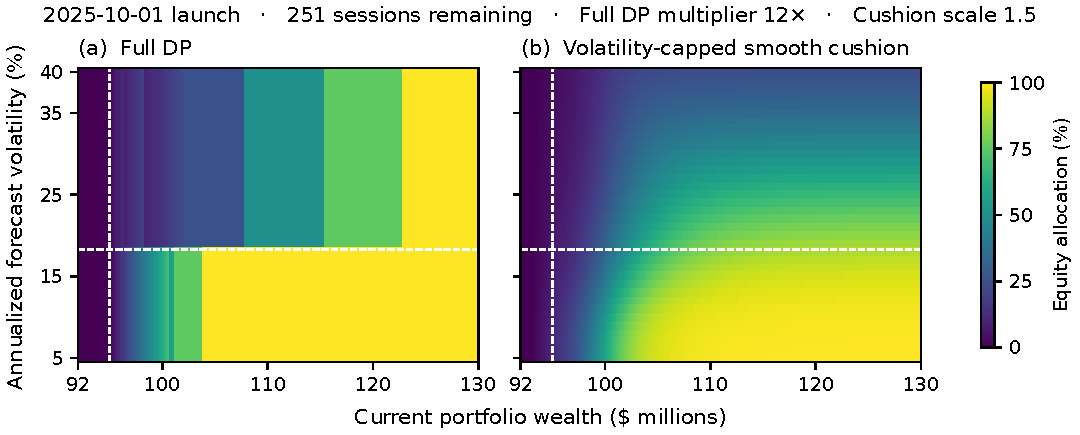
\includegraphics[width=0.93\textwidth]{figures/smooth-wealth-volatility.pdf}
 \caption{Equity weights for the same October 2025 launch and wealth--volatility grid as Figure~\ref{fig:ccdp-vol}. The vertical line marks the nominal terminal floor. The horizontal line marks the DP regime cutoff, shown on both panels for reference. Both policies retain their launch settings.}
 \label{fig:smooth-vol}
\end{figure*}

\begin{figure*}[tbp]
 \centering
 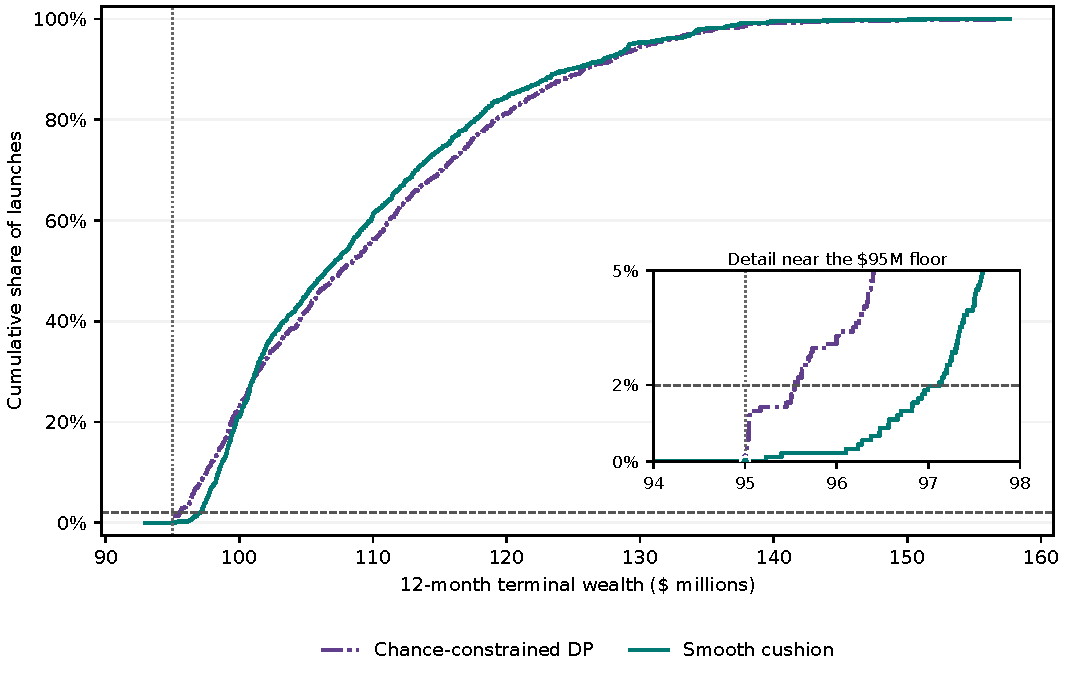
\includegraphics[width=0.87\textwidth]{figures/smooth-terminal-cdf.pdf}
 \caption{Terminal wealth for the chance-constrained DP and smooth cushion on the same 910 monthly launches as Figure~\ref{fig:ccdp-cdf}. The inset shows the share finishing at or below each wealth level from \$94 to \$98 million. Dots mark the share at \$95 million and the horizontal dashed line marks 2\%.}
 \label{fig:smooth-cdf}
\end{figure*}
; keep the figures/ subdirectory alongside the main
% manuscript or add their directory to \graphicspath. Requires amsmath,
% amssymb, and graphicx.
\subsection{The standard dynamic programming model}
We consider a portfolio with initial wealth $W_0=\$100$ million and a nominal terminal floor $F=\$95$ million. At each trading session $t$, the investor observes wealth $W_t$ and a volatility regime $z_t$, and allocates a fraction $a_t\in\mathcal A_0=\{0,0.25,0.50,0.75,1\}$ to equity. The balance earns the daily cash rate $r_f=0.02/252$. If $X_{t+1}$ denotes the equity return in excess of cash, wealth evolves as $W_{t+1}=W_t(1+r_f+a_tX_{t+1})$.

The high-volatility regime applies when the pre-trade volatility forecast exceeds its historical 80th percentile. In the planning model, the two equally likely excess returns are $\mu\pm\sigma_z/\sqrt{252}$, where $\mu=0.05/252$ and annual volatility is $0.15$ in the ordinary regime and $0.30$ in the high regime. The regime switches independently of the return shock, with daily transition probabilities of $0.01$ from ordinary to high and $0.04$ from high to ordinary.

The investor values terminal wealth through $u(x)=-1/x-5(0.95-x)^+$, where $x=W_T/W_0$ and $y^+=\max(y,0)$. The second term penalizes the magnitude of a terminal shortfall. Starting from $V_T(w,z)=u(w/W_0)$, backward induction gives
\begin{equation}
 V_t(w,z)=\max_{a\in\mathcal A_0}
 \mathbb E\!\left[V_{t+1}\bigl(w(1+r_f+aX_{t+1}),z_{t+1}\bigr)\mid z_t=z\right].
\end{equation}

\subsection{Chance-constrained dynamic programming}
We extend the baseline model to pursue higher mean terminal wealth while keeping the modeled probability of finishing below the floor under 2\%.
\paragraph{Wealth-dependent equity cap.}
The baseline model allows full equity exposure even when wealth is just above the floor. We cap equity exposure according to the dollar cushion $C(w)=(w-F)^+$. The cap allows $m$ dollars of equity exposure per dollar of cushion up to $K=\$5$ million, and $1.5m$ dollars per additional dollar of cushion. Total equity exposure is bounded by
\begin{equation}
 E_{\max}(w)=\min\!\left\{w,\;m\min(C(w),K)+1.5m\bigl(C(w)-K\bigr)^+\right\}.
\end{equation}
The admissible dollar positions comprise the baseline positions $aw$, $a\in\mathcal A_0$, clipped to $E_{\max}(w)$, together with 25\%, 50\%, and 75\% of the cap. These intermediate positions preserve allocation choices near the floor, where several baseline positions collapse to the same cap. At or below the floor, the portfolio holds cash. Each launch retains the multiplier selected for its opening year using only previously completed investments.

\paragraph{Rare downside shocks.}
A sharp one-day loss can exhaust the cushion even when the equity position satisfies the cap. To capture this risk, we add a rare downside shock to each regime. The model assigns a daily probability $p_z$ to an excess return $g_z$, with $(p_z,g_z)=(0.001,-0.10)$ in the ordinary regime and $(0.004,-0.20)$ in the high regime. The remaining two outcomes, $c_z\pm\sigma_z/\sqrt{252}$, each receive probability $(1-p_z)/2$. Choosing $c_z=(\mu-p_zg_z)/(1-p_z)$ preserves the baseline expected equity premium.

\paragraph{Terminal probability constraint.}
The baseline utility penalizes the size of a shortfall but places no limit on its probability. We impose that limit directly and maximize expected terminal wealth subject to it. For the launch state $s_0=(W_0,z_0)$ and the prescribed maturity $T$, the target problem is
\begin{equation}
 \max_{\pi}\;\mathbb E_{\pi}[W_T\mid s_0]
 \quad\text{subject to}\quad
 \Pr_{\pi}(W_T<F\mid s_0)<0.02 .
\end{equation}
We approximate this problem with four candidate policies and an all-cash alternative. For each breach penalty $\lambda\in\{0,10,100,1000\}$ million dollars, backward induction uses the terminal payoff $W_T-\lambda\mathbf{1}_{\{W_T<F\}}$ and tracks both expected terminal wealth and breach probability under the resulting policy. At launch, the strategy selects the candidate with the highest modeled mean among those satisfying the probability limit. The selected policy remains fixed through maturity, while its equity allocation responds daily to wealth, regime, and time remaining.

Figures~\ref{fig:ccdp-vol} and~\ref{fig:ccdp-cdf} show the allocation rules and historical terminal wealth distributions for the four cumulative specifications. The first three maximize the original terminal utility, which isolates the effect of changing the action set and then the transition law. The fourth introduces the constrained mean-wealth objective. All four use realized equity and cash returns in the historical replay. Across 910 launches, the equity cap reduces the number of terminal breaches from 34 to one. Each subsequent specification also records one breach. Under the gap model, replacing terminal utility with the constrained mean-wealth objective raises historical mean terminal wealth from \$109.11 million to \$109.85 million.

\begin{figure*}[tbp]
 \centering
 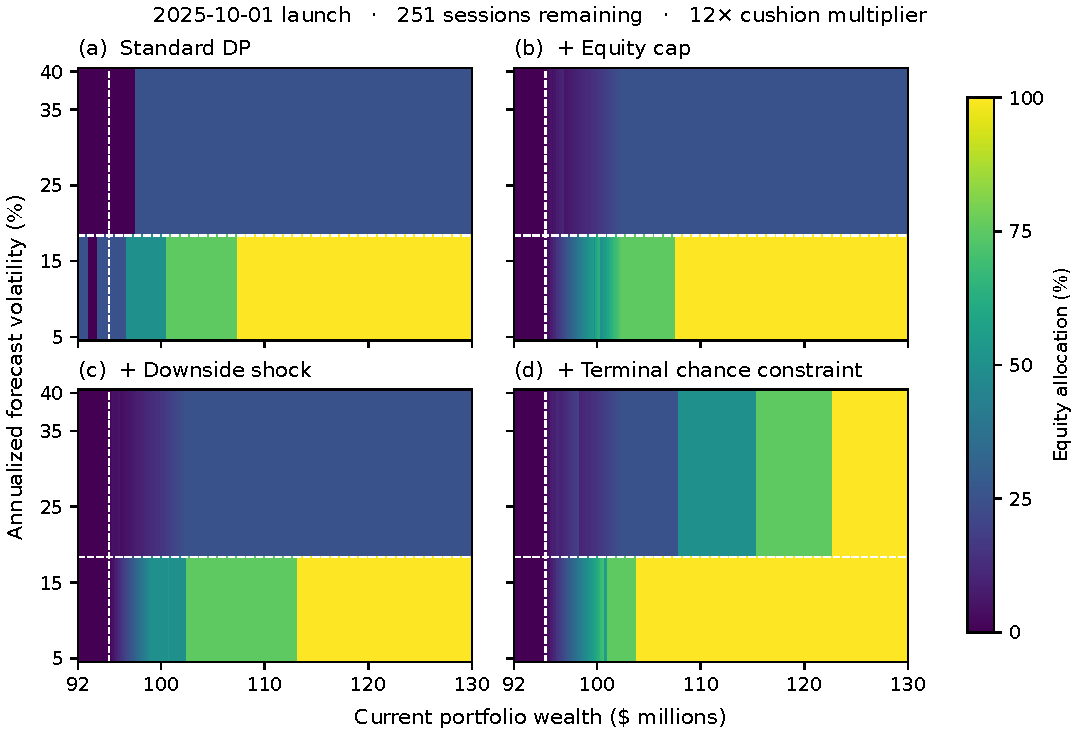
\includegraphics[width=0.93\textwidth]{figures/wealth-volatility.pdf}
 \caption{Equity allocation as a function of current wealth and forecast volatility for the latest eligible 12-month launch. Each panel quotes a strategy at the same remaining horizon. Color gives the percentage of wealth invested in equity. The vertical dashed line marks the \$95 million floor and the horizontal dashed line marks the launch volatility cutoff. Panel (d) retains the policy selected at launch across all plotted states.}
 \label{fig:ccdp-vol}
\end{figure*}

\begin{figure*}[tbp]
 \centering
 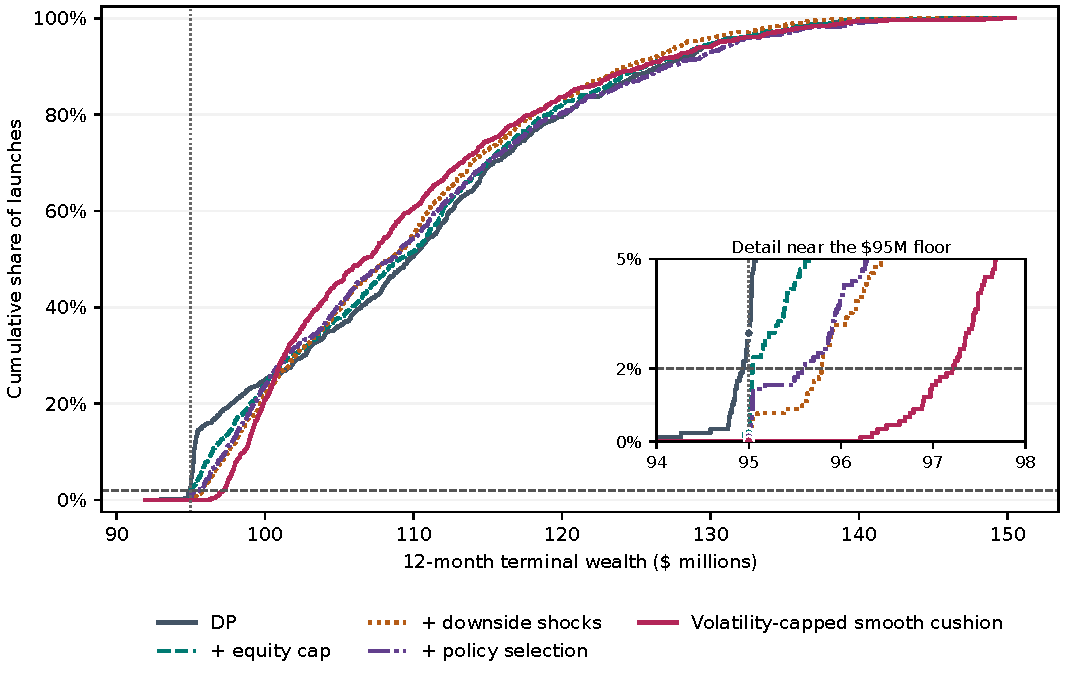
\includegraphics[width=0.87\textwidth]{figures/terminal-cdf.pdf}
 \caption{Empirical cumulative distributions of terminal wealth for 910 overlapping 12-month investments launched monthly from January 1950 through October 2025. At each wealth level, the curve gives the fraction of launches ending at or below that level. The inset spans \$94--96 million and cumulative probabilities from 0 to 5\%. Dots mark the empirical CDF at \$95 million. The three capped strategies coincide there. Horizontal dashed lines mark 2\%. The left limit at the \$95 million floor gives the historical terminal breach rate. The 2\% policy limit applies to the modeled probability at launch.}
 \label{fig:ccdp-cdf}
\end{figure*}


\subsection{Smooth Variant}
The chance-constrained DP heatmap suggests a simpler daily rule. Moving right in Figure~\ref{fig:ccdp-vol}(d), a larger cushion supports more equity. Moving upward, even a small change in forecast volatility can switch the regime and abruptly change the position. The smooth variant preserves the cushion response and uses the volatility forecast directly to reduce exposure gradually.

\paragraph{Why discount the floor?}
At \$100 million of wealth and 15\% forecast volatility, the October 2025 DP policy allocates 60\% to equity with 251 sessions left and 50\% with one session left. The smooth rule captures this horizon effect through the cost of funding the floor. At the modeled cash rate, the reserve needed to fund \$95 million at maturity rises from \$93.13 million to \$94.99 million between those dates. At the same wealth, this leaves \$6.87 million of cushion early in the year and only \$5.01 million on the final trading day.

\paragraph{Daily allocation.}
Measure wealth in millions of dollars. With $n=T-t$ sessions remaining, the reserve is $F_n=F(1+r_f)^{-n}$ and the cushion is $c=(W_t-F_n)^+$. Define base equity exposure by $G(c)=\int_0^c h(u)\,du$, where
\[
 h(u)=1+\frac{(u-3)^+-(u-7)^+}{2}
       +\frac{(u-15)^+-(u-25)^+}{10}.
\]
Each additional cushion dollar initially supports one dollar of base equity exposure. Its contribution rises gradually to three dollars over the \$3--7 million band and to four over the \$15--25 million band.

For annualized forecast volatility $v$ and launch scale $s$, the rule reduces the requested equity fraction $r$ as volatility rises and sets a ceiling $L(v)$ according to
\[
 r=1.25\,s\,\frac{3}{[1+(v/0.10)^6]^{1/6}}\frac{G(c)}{W_t},
 \qquad L(v)=\frac{1}{1+(v/0.30)^4}.
\]
Each session the strategy rebalances to equity holdings of $a_t W_t$, where the target fraction is
\[
 a_t=\frac{r}{[1+(r/L(v))^4]^{1/4}}.
\]
Near the reserve, the rule grants approximately the requested fraction. With ample cushion, the weight approaches the volatility ceiling, which falls from 50\% at 30\% volatility to 24\% at 40\% volatility (Figure~\ref{fig:smooth-vol}). The breakpoints and ceiling are design choices motivated by the DP surface. Each one-year launch inherits the scale selected on completed launches for the earlier time-aware cushion rule. During sparse-history warm-up it uses unit scale and the nominal floor.

Table~\ref{tab:strategy-overview} compares all five strategies on the same 12-month launches. Table~\ref{tab:strategy-comparison} then compares the final two strategies on the committee's objective and floor. The chance-constrained DP achieved higher overall certainty-equivalent wealth at both horizons, while the smooth rule achieved higher certainty-equivalent wealth on crisis launches at both horizons. Of these two strategies, only the DP breached the floor, on one lower-volatility 12-month launch. Over all 12-month launches, the worst finish was \$94.996 million for the DP and \$95.230 million for the smooth rule. Figure~\ref{fig:smooth-cdf} shows the crossing distributions near the floor.

\begin{table*}[tbp]
 \centering
 \caption{Certainty-equivalent wealth, mean terminal wealth, and floor breaches for 910 overlapping 12-month investments of \$100 million each, launched monthly from January 1950 through October 2025. A launch is classified as crisis if the equity total-return index closed at least 20\% below its trailing 12-month high on the previous trading day. For all other launches, higher volatility means that the volatility of daily equity returns over the preceding 63 trading sessions exceeded the median across all earlier 63-session windows. Lower volatility includes values at or below that median.}
 \label{tab:strategy-overview}
 \small
 \begin{tabular}{@{}lrrr@{}}
\hline
Strategy & Objective: CE (\$M) & Mean $W_T$ (\$M) & Breaches (\%) \\
\hline
\multicolumn{4}{@{}l}{\itshape All launches ($n=910$)} \\
Standard DP & 108.87 & \textbf{110.04} & 34 (3.74\%) \\
DP with equity cap & 108.60 & 109.55 & 1 (0.11\%) \\
Capped DP with downside shocks & 108.26 & 109.11 & 1 (0.11\%) \\
Chance-constrained DP & \textbf{108.80} & 109.85 & 1 (0.11\%) \\
Smooth cushion & 108.24 & 109.16 & \textbf{0 (0.00\%)} \\
\hline
\multicolumn{4}{@{}l}{\itshape Lower volatility ($n=440$)} \\
Standard DP & 108.98 & \textbf{110.15} & 9 (2.05\%) \\
DP with equity cap & 108.64 & 109.58 & 1 (0.23\%) \\
Capped DP with downside shocks & 108.44 & 109.29 & \textbf{0 (0.00\%)} \\
Chance-constrained DP & \textbf{108.77} & 109.77 & 1 (0.23\%) \\
Smooth cushion & 108.28 & 109.20 & \textbf{0 (0.00\%)} \\
\hline
\multicolumn{4}{@{}l}{\itshape Higher volatility ($n=416$)} \\
Standard DP & 108.62 & \textbf{109.78} & 24 (5.77\%) \\
DP with equity cap & 108.46 & 109.42 & \textbf{0 (0.00\%)} \\
Capped DP with downside shocks & 107.98 & 108.83 & 1 (0.24\%) \\
Chance-constrained DP & \textbf{108.64} & 109.75 & \textbf{0 (0.00\%)} \\
Smooth cushion & 107.89 & 108.82 & \textbf{0 (0.00\%)} \\
\hline
\multicolumn{4}{@{}l}{\itshape Crisis ($n=54$)} \\
Standard DP & 109.93 & 111.03 & 1 (1.85\%) \\
DP with equity cap & 109.41 & 110.30 & \textbf{0 (0.00\%)} \\
Capped DP with downside shocks & 109.00 & 109.79 & \textbf{0 (0.00\%)} \\
Chance-constrained DP & 110.36 & 111.35 & \textbf{0 (0.00\%)} \\
Smooth cushion & \textbf{110.67} & \textbf{111.56} & \textbf{0 (0.00\%)} \\
\hline
\end{tabular}

 \par\smallskip
 \begin{minipage}{0.96\linewidth}\footnotesize
 For each launch group, the objective value at $\gamma=2$ is $\mathrm{CE}=(n^{-1}\sum_{i=1}^{n}1/W_{T,i})^{-1}$. Breaches count finishes strictly below \$95 million. Percentages use the same group. Within each group, bold marks the highest CE among strategies with observed breach rates at or below 2\% in every launch condition, the highest arithmetic mean, and the fewest breaches (including ties).
 \end{minipage}
\end{table*}

\begin{table*}[tbp]
 \centering
 \caption{Historical certainty-equivalent terminal wealth and floor breaches from a \$100 million investment, by market condition at launch.}
 \label{tab:strategy-comparison}
 \small
 \begin{tabular}{@{}llrrrrr@{}}
\hline
& & & \multicolumn{2}{c}{Chance-constrained DP} & \multicolumn{2}{c}{Smooth cushion} \\
\cline{4-5}\cline{6-7}
Horizon & Launch condition & Launches & CE (\$M) & Breaches (\%) & CE (\$M) & Breaches (\%) \\
\hline
12 months & All launches & 910 & 108.80 & 1 (0.11\%) & 108.24 & 0 (0\%) \\
 & Lower volatility & 440 & 108.77 & 1 (0.23\%) & 108.28 & 0 (0\%) \\
 & Higher volatility & 416 & 108.64 & 0 (0\%) & 107.89 & 0 (0\%) \\
 & Crisis & 54 & 110.36 & 0 (0\%) & 110.67 & 0 (0\%) \\
\hline
24 months & All launches & 898 & 117.90 & 0 (0\%) & 116.57 & 0 (0\%) \\
 & Lower volatility & 438 & 119.36 & 0 (0\%) & 117.88 & 0 (0\%) \\
 & Higher volatility & 406 & 115.86 & 0 (0\%) & 114.44 & 0 (0\%) \\
 & Crisis & 54 & 121.94 & 0 (0\%) & 122.79 & 0 (0\%) \\
\hline
\end{tabular}

 \par\smallskip
 \begin{minipage}{0.96\linewidth}\footnotesize
 CE is the harmonic mean of terminal wealth ($\gamma=2$). Breaches count launches finishing strictly below \$95 million, with the observed rate in parentheses. Monthly launches overlap, so these rates alone cannot establish a 2\% upper bound on breach probability. The smooth rule uses its historically selected scale at 12 months and a fixed scale of one at 24 months.
 \end{minipage}
\end{table*}

\begin{figure*}[tbp]
 \centering
 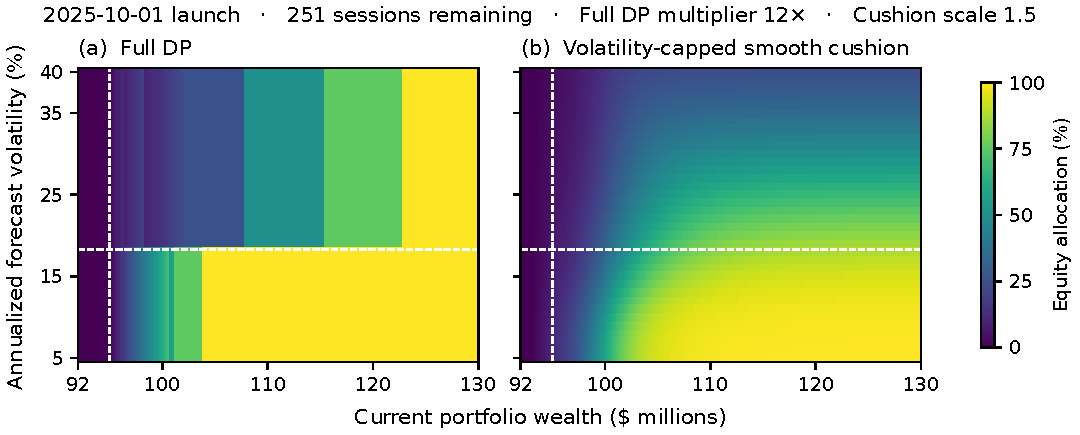
\includegraphics[width=0.93\textwidth]{figures/smooth-wealth-volatility.pdf}
 \caption{Equity weights for the same October 2025 launch and wealth--volatility grid as Figure~\ref{fig:ccdp-vol}. The vertical line marks the nominal terminal floor. The horizontal line marks the DP regime cutoff, shown on both panels for reference. Both policies retain their launch settings.}
 \label{fig:smooth-vol}
\end{figure*}

\begin{figure*}[tbp]
 \centering
 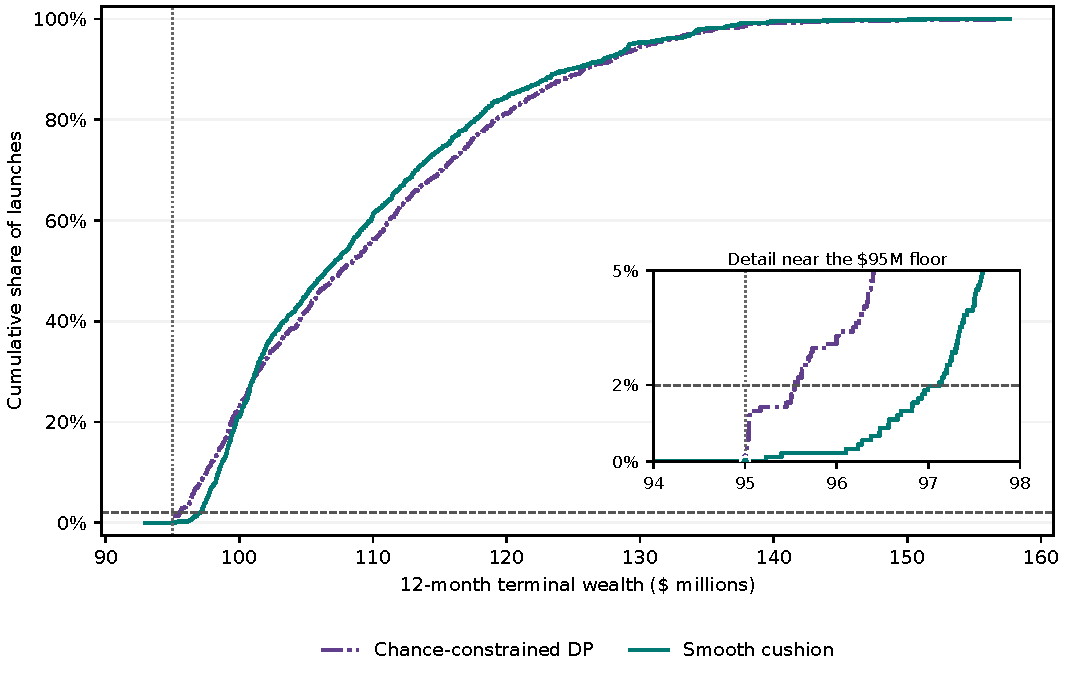
\includegraphics[width=0.87\textwidth]{figures/smooth-terminal-cdf.pdf}
 \caption{Terminal wealth for the chance-constrained DP and smooth cushion on the same 910 monthly launches as Figure~\ref{fig:ccdp-cdf}. The inset shows the share finishing at or below each wealth level from \$94 to \$98 million. Dots mark the share at \$95 million and the horizontal dashed line marks 2\%.}
 \label{fig:smooth-cdf}
\end{figure*}
; keep the figures/ subdirectory alongside the main
% manuscript or add their directory to \graphicspath. Requires amsmath,
% amssymb, and graphicx.
\subsection{The standard dynamic programming model}
We consider a portfolio with initial wealth $W_0=\$100$ million and a nominal terminal floor $F=\$95$ million. At each trading session $t$, the investor observes wealth $W_t$ and a volatility regime $z_t$, and allocates a fraction $a_t\in\mathcal A_0=\{0,0.25,0.50,0.75,1\}$ to equity. The balance earns the daily cash rate $r_f=0.02/252$. If $X_{t+1}$ denotes the equity return in excess of cash, wealth evolves as $W_{t+1}=W_t(1+r_f+a_tX_{t+1})$.

The high-volatility regime applies when the pre-trade volatility forecast exceeds its historical 80th percentile. In the planning model, the two equally likely excess returns are $\mu\pm\sigma_z/\sqrt{252}$, where $\mu=0.05/252$ and annual volatility is $0.15$ in the ordinary regime and $0.30$ in the high regime. The regime switches independently of the return shock, with daily transition probabilities of $0.01$ from ordinary to high and $0.04$ from high to ordinary.

The investor values terminal wealth through $u(x)=-1/x-5(0.95-x)^+$, where $x=W_T/W_0$ and $y^+=\max(y,0)$. The second term penalizes the magnitude of a terminal shortfall. Starting from $V_T(w,z)=u(w/W_0)$, backward induction gives
\begin{equation}
 V_t(w,z)=\max_{a\in\mathcal A_0}
 \mathbb E\!\left[V_{t+1}\bigl(w(1+r_f+aX_{t+1}),z_{t+1}\bigr)\mid z_t=z\right].
\end{equation}

\subsection{Chance-constrained dynamic programming}
We extend the baseline model to pursue higher mean terminal wealth while keeping the modeled probability of finishing below the floor under 2\%.
\paragraph{Wealth-dependent equity cap.}
The baseline model allows full equity exposure even when wealth is just above the floor. We cap equity exposure according to the dollar cushion $C(w)=(w-F)^+$. The cap allows $m$ dollars of equity exposure per dollar of cushion up to $K=\$5$ million, and $1.5m$ dollars per additional dollar of cushion. Total equity exposure is bounded by
\begin{equation}
 E_{\max}(w)=\min\!\left\{w,\;m\min(C(w),K)+1.5m\bigl(C(w)-K\bigr)^+\right\}.
\end{equation}
The admissible dollar positions comprise the baseline positions $aw$, $a\in\mathcal A_0$, clipped to $E_{\max}(w)$, together with 25\%, 50\%, and 75\% of the cap. These intermediate positions preserve allocation choices near the floor, where several baseline positions collapse to the same cap. At or below the floor, the portfolio holds cash. Each launch retains the multiplier selected for its opening year using only previously completed investments.

\paragraph{Rare downside shocks.}
A sharp one-day loss can exhaust the cushion even when the equity position satisfies the cap. To capture this risk, we add a rare downside shock to each regime. The model assigns a daily probability $p_z$ to an excess return $g_z$, with $(p_z,g_z)=(0.001,-0.10)$ in the ordinary regime and $(0.004,-0.20)$ in the high regime. The remaining two outcomes, $c_z\pm\sigma_z/\sqrt{252}$, each receive probability $(1-p_z)/2$. Choosing $c_z=(\mu-p_zg_z)/(1-p_z)$ preserves the baseline expected equity premium.

\paragraph{Terminal probability constraint.}
The baseline utility penalizes the size of a shortfall but places no limit on its probability. We impose that limit directly and maximize expected terminal wealth subject to it. For the launch state $s_0=(W_0,z_0)$ and the prescribed maturity $T$, the target problem is
\begin{equation}
 \max_{\pi}\;\mathbb E_{\pi}[W_T\mid s_0]
 \quad\text{subject to}\quad
 \Pr_{\pi}(W_T<F\mid s_0)<0.02 .
\end{equation}
We approximate this problem with four candidate policies and an all-cash alternative. For each breach penalty $\lambda\in\{0,10,100,1000\}$ million dollars, backward induction uses the terminal payoff $W_T-\lambda\mathbf{1}_{\{W_T<F\}}$ and tracks both expected terminal wealth and breach probability under the resulting policy. At launch, the strategy selects the candidate with the highest modeled mean among those satisfying the probability limit. The selected policy remains fixed through maturity, while its equity allocation responds daily to wealth, regime, and time remaining.

Figures~\ref{fig:ccdp-vol} and~\ref{fig:ccdp-cdf} show the allocation rules and historical terminal wealth distributions for the four cumulative specifications. The first three maximize the original terminal utility, which isolates the effect of changing the action set and then the transition law. The fourth introduces the constrained mean-wealth objective. All four use realized equity and cash returns in the historical replay. Across 910 launches, the equity cap reduces the number of terminal breaches from 34 to one. Each subsequent specification also records one breach. Under the gap model, replacing terminal utility with the constrained mean-wealth objective raises historical mean terminal wealth from \$109.11 million to \$109.85 million.

\begin{figure*}[tbp]
 \centering
 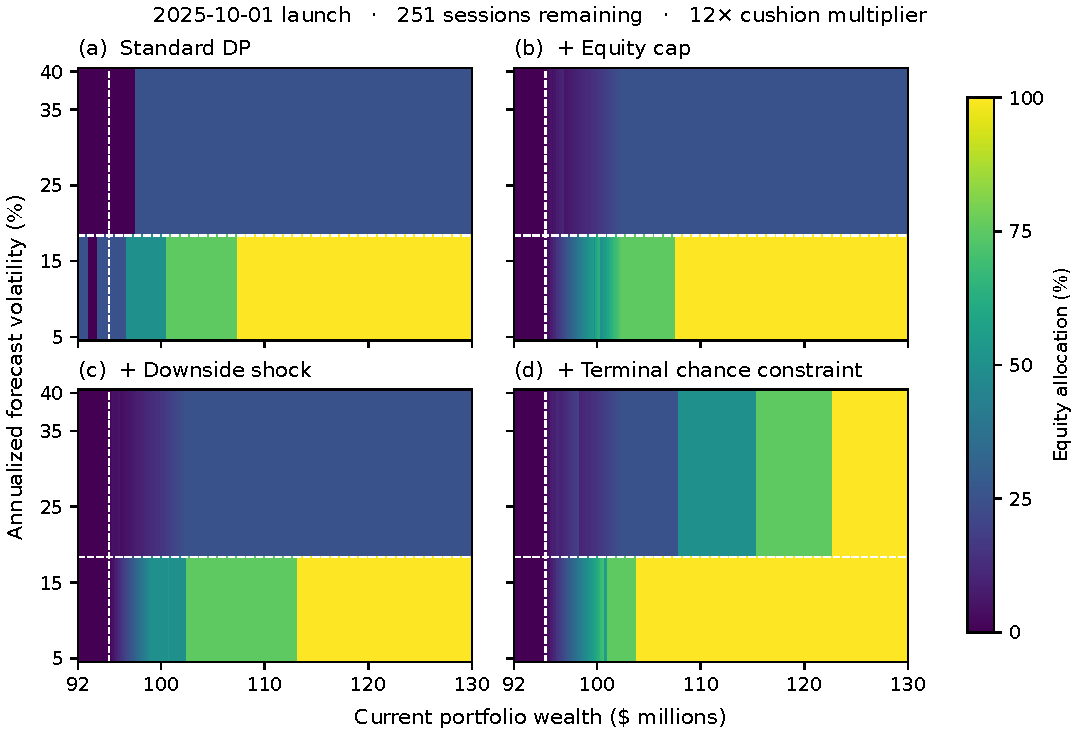
\includegraphics[width=0.93\textwidth]{figures/wealth-volatility.pdf}
 \caption{Equity allocation as a function of current wealth and forecast volatility for the latest eligible 12-month launch. Each panel quotes a strategy at the same remaining horizon. Color gives the percentage of wealth invested in equity. The vertical dashed line marks the \$95 million floor and the horizontal dashed line marks the launch volatility cutoff. Panel (d) retains the policy selected at launch across all plotted states.}
 \label{fig:ccdp-vol}
\end{figure*}

\begin{figure*}[tbp]
 \centering
 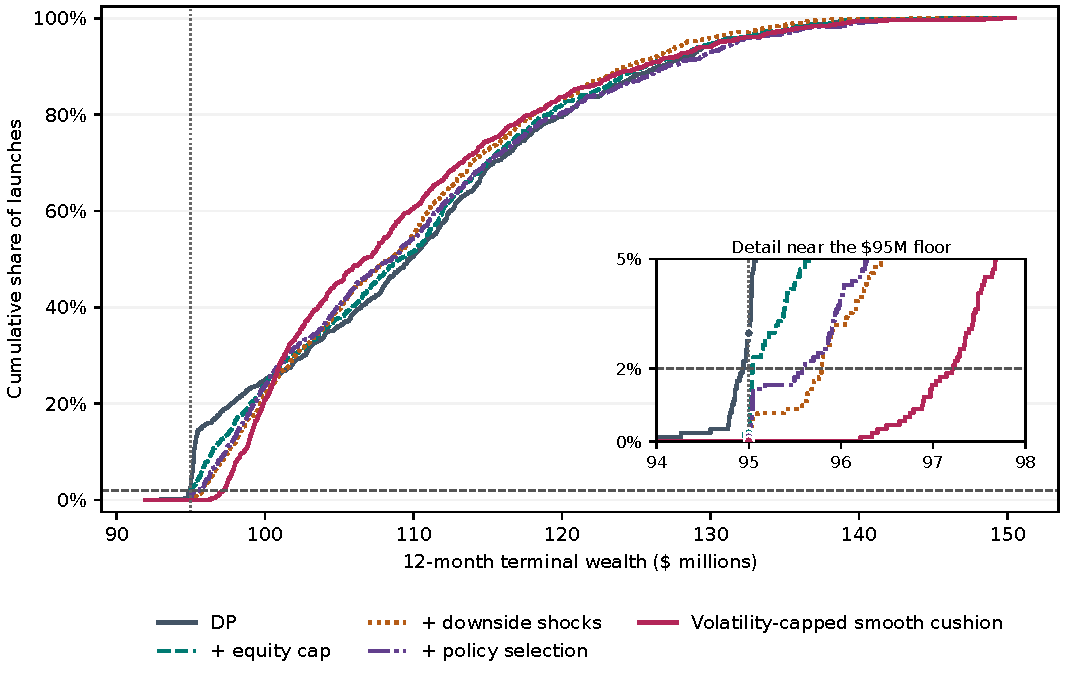
\includegraphics[width=0.87\textwidth]{figures/terminal-cdf.pdf}
 \caption{Empirical cumulative distributions of terminal wealth for 910 overlapping 12-month investments launched monthly from January 1950 through October 2025. At each wealth level, the curve gives the fraction of launches ending at or below that level. The inset spans \$94--96 million and cumulative probabilities from 0 to 5\%. Dots mark the empirical CDF at \$95 million. The three capped strategies coincide there. Horizontal dashed lines mark 2\%. The left limit at the \$95 million floor gives the historical terminal breach rate. The 2\% policy limit applies to the modeled probability at launch.}
 \label{fig:ccdp-cdf}
\end{figure*}


\subsection{Smooth Variant}
The chance-constrained DP heatmap suggests a simpler daily rule. Moving right in Figure~\ref{fig:ccdp-vol}(d), a larger cushion supports more equity. Moving upward, even a small change in forecast volatility can switch the regime and abruptly change the position. The smooth variant preserves the cushion response and uses the volatility forecast directly to reduce exposure gradually.

\paragraph{Why discount the floor?}
At \$100 million of wealth and 15\% forecast volatility, the October 2025 DP policy allocates 60\% to equity with 251 sessions left and 50\% with one session left. The smooth rule captures this horizon effect through the cost of funding the floor. At the modeled cash rate, the reserve needed to fund \$95 million at maturity rises from \$93.13 million to \$94.99 million between those dates. At the same wealth, this leaves \$6.87 million of cushion early in the year and only \$5.01 million on the final trading day.

\paragraph{Daily allocation.}
Measure wealth in millions of dollars. With $n=T-t$ sessions remaining, the reserve is $F_n=F(1+r_f)^{-n}$ and the cushion is $c=(W_t-F_n)^+$. Define base equity exposure by $G(c)=\int_0^c h(u)\,du$, where
\[
 h(u)=1+\frac{(u-3)^+-(u-7)^+}{2}
       +\frac{(u-15)^+-(u-25)^+}{10}.
\]
Each additional cushion dollar initially supports one dollar of base equity exposure. Its contribution rises gradually to three dollars over the \$3--7 million band and to four over the \$15--25 million band.

For annualized forecast volatility $v$ and launch scale $s$, the rule reduces the requested equity fraction $r$ as volatility rises and sets a ceiling $L(v)$ according to
\[
 r=1.25\,s\,\frac{3}{[1+(v/0.10)^6]^{1/6}}\frac{G(c)}{W_t},
 \qquad L(v)=\frac{1}{1+(v/0.30)^4}.
\]
Each session the strategy rebalances to equity holdings of $a_t W_t$, where the target fraction is
\[
 a_t=\frac{r}{[1+(r/L(v))^4]^{1/4}}.
\]
Near the reserve, the rule grants approximately the requested fraction. With ample cushion, the weight approaches the volatility ceiling, which falls from 50\% at 30\% volatility to 24\% at 40\% volatility (Figure~\ref{fig:smooth-vol}). The breakpoints and ceiling are design choices motivated by the DP surface. Each one-year launch inherits the scale selected on completed launches for the earlier time-aware cushion rule. During sparse-history warm-up it uses unit scale and the nominal floor.

Table~\ref{tab:strategy-overview} compares all five strategies on the same 12-month launches. Table~\ref{tab:strategy-comparison} then compares the final two strategies on the committee's objective and floor. The chance-constrained DP achieved higher overall certainty-equivalent wealth at both horizons, while the smooth rule achieved higher certainty-equivalent wealth on crisis launches at both horizons. Of these two strategies, only the DP breached the floor, on one lower-volatility 12-month launch. Over all 12-month launches, the worst finish was \$94.996 million for the DP and \$95.230 million for the smooth rule. Figure~\ref{fig:smooth-cdf} shows the crossing distributions near the floor.

\begin{table*}[tbp]
 \centering
 \caption{Certainty-equivalent wealth, mean terminal wealth, and floor breaches for 910 overlapping 12-month investments of \$100 million each, launched monthly from January 1950 through October 2025. A launch is classified as crisis if the equity total-return index closed at least 20\% below its trailing 12-month high on the previous trading day. For all other launches, higher volatility means that the volatility of daily equity returns over the preceding 63 trading sessions exceeded the median across all earlier 63-session windows. Lower volatility includes values at or below that median.}
 \label{tab:strategy-overview}
 \small
 \begin{tabular}{@{}lrrr@{}}
\hline
Strategy & Objective: CE (\$M) & Mean $W_T$ (\$M) & Breaches (\%) \\
\hline
\multicolumn{4}{@{}l}{\itshape All launches ($n=910$)} \\
Standard DP & 108.87 & \textbf{110.04} & 34 (3.74\%) \\
DP with equity cap & 108.60 & 109.55 & 1 (0.11\%) \\
Capped DP with downside shocks & 108.26 & 109.11 & 1 (0.11\%) \\
Chance-constrained DP & \textbf{108.80} & 109.85 & 1 (0.11\%) \\
Smooth cushion & 108.24 & 109.16 & \textbf{0 (0.00\%)} \\
\hline
\multicolumn{4}{@{}l}{\itshape Lower volatility ($n=440$)} \\
Standard DP & 108.98 & \textbf{110.15} & 9 (2.05\%) \\
DP with equity cap & 108.64 & 109.58 & 1 (0.23\%) \\
Capped DP with downside shocks & 108.44 & 109.29 & \textbf{0 (0.00\%)} \\
Chance-constrained DP & \textbf{108.77} & 109.77 & 1 (0.23\%) \\
Smooth cushion & 108.28 & 109.20 & \textbf{0 (0.00\%)} \\
\hline
\multicolumn{4}{@{}l}{\itshape Higher volatility ($n=416$)} \\
Standard DP & 108.62 & \textbf{109.78} & 24 (5.77\%) \\
DP with equity cap & 108.46 & 109.42 & \textbf{0 (0.00\%)} \\
Capped DP with downside shocks & 107.98 & 108.83 & 1 (0.24\%) \\
Chance-constrained DP & \textbf{108.64} & 109.75 & \textbf{0 (0.00\%)} \\
Smooth cushion & 107.89 & 108.82 & \textbf{0 (0.00\%)} \\
\hline
\multicolumn{4}{@{}l}{\itshape Crisis ($n=54$)} \\
Standard DP & 109.93 & 111.03 & 1 (1.85\%) \\
DP with equity cap & 109.41 & 110.30 & \textbf{0 (0.00\%)} \\
Capped DP with downside shocks & 109.00 & 109.79 & \textbf{0 (0.00\%)} \\
Chance-constrained DP & 110.36 & 111.35 & \textbf{0 (0.00\%)} \\
Smooth cushion & \textbf{110.67} & \textbf{111.56} & \textbf{0 (0.00\%)} \\
\hline
\end{tabular}

 \par\smallskip
 \begin{minipage}{0.96\linewidth}\footnotesize
 For each launch group, the objective value at $\gamma=2$ is $\mathrm{CE}=(n^{-1}\sum_{i=1}^{n}1/W_{T,i})^{-1}$. Breaches count finishes strictly below \$95 million. Percentages use the same group. Within each group, bold marks the highest CE among strategies with observed breach rates at or below 2\% in every launch condition, the highest arithmetic mean, and the fewest breaches (including ties).
 \end{minipage}
\end{table*}

\begin{table*}[tbp]
 \centering
 \caption{Historical certainty-equivalent terminal wealth and floor breaches from a \$100 million investment, by market condition at launch.}
 \label{tab:strategy-comparison}
 \small
 \begin{tabular}{@{}llrrrrr@{}}
\hline
& & & \multicolumn{2}{c}{Chance-constrained DP} & \multicolumn{2}{c}{Smooth cushion} \\
\cline{4-5}\cline{6-7}
Horizon & Launch condition & Launches & CE (\$M) & Breaches (\%) & CE (\$M) & Breaches (\%) \\
\hline
12 months & All launches & 910 & 108.80 & 1 (0.11\%) & 108.24 & 0 (0\%) \\
 & Lower volatility & 440 & 108.77 & 1 (0.23\%) & 108.28 & 0 (0\%) \\
 & Higher volatility & 416 & 108.64 & 0 (0\%) & 107.89 & 0 (0\%) \\
 & Crisis & 54 & 110.36 & 0 (0\%) & 110.67 & 0 (0\%) \\
\hline
24 months & All launches & 898 & 117.90 & 0 (0\%) & 116.57 & 0 (0\%) \\
 & Lower volatility & 438 & 119.36 & 0 (0\%) & 117.88 & 0 (0\%) \\
 & Higher volatility & 406 & 115.86 & 0 (0\%) & 114.44 & 0 (0\%) \\
 & Crisis & 54 & 121.94 & 0 (0\%) & 122.79 & 0 (0\%) \\
\hline
\end{tabular}

 \par\smallskip
 \begin{minipage}{0.96\linewidth}\footnotesize
 CE is the harmonic mean of terminal wealth ($\gamma=2$). Breaches count launches finishing strictly below \$95 million, with the observed rate in parentheses. Monthly launches overlap, so these rates alone cannot establish a 2\% upper bound on breach probability. The smooth rule uses its historically selected scale at 12 months and a fixed scale of one at 24 months.
 \end{minipage}
\end{table*}

\begin{figure*}[tbp]
 \centering
 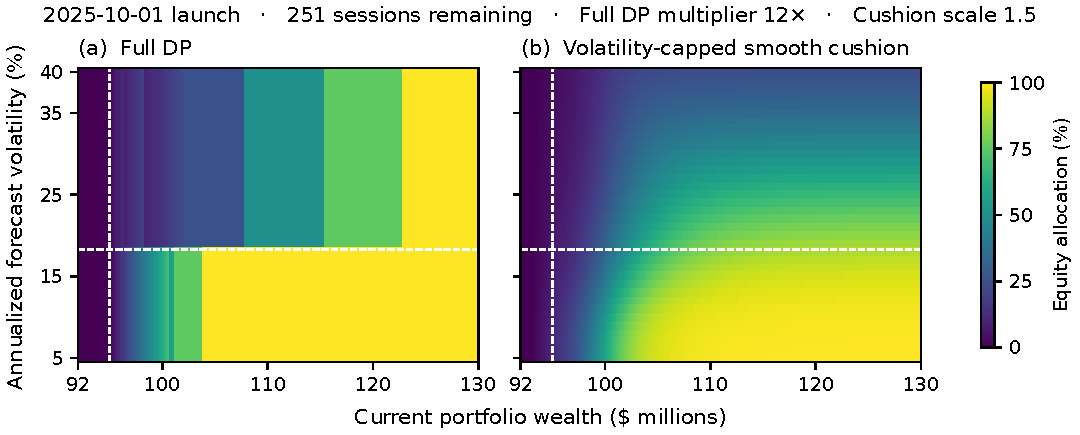
\includegraphics[width=0.93\textwidth]{figures/smooth-wealth-volatility.pdf}
 \caption{Equity weights for the same October 2025 launch and wealth--volatility grid as Figure~\ref{fig:ccdp-vol}. The vertical line marks the nominal terminal floor. The horizontal line marks the DP regime cutoff, shown on both panels for reference. Both policies retain their launch settings.}
 \label{fig:smooth-vol}
\end{figure*}

\begin{figure*}[tbp]
 \centering
 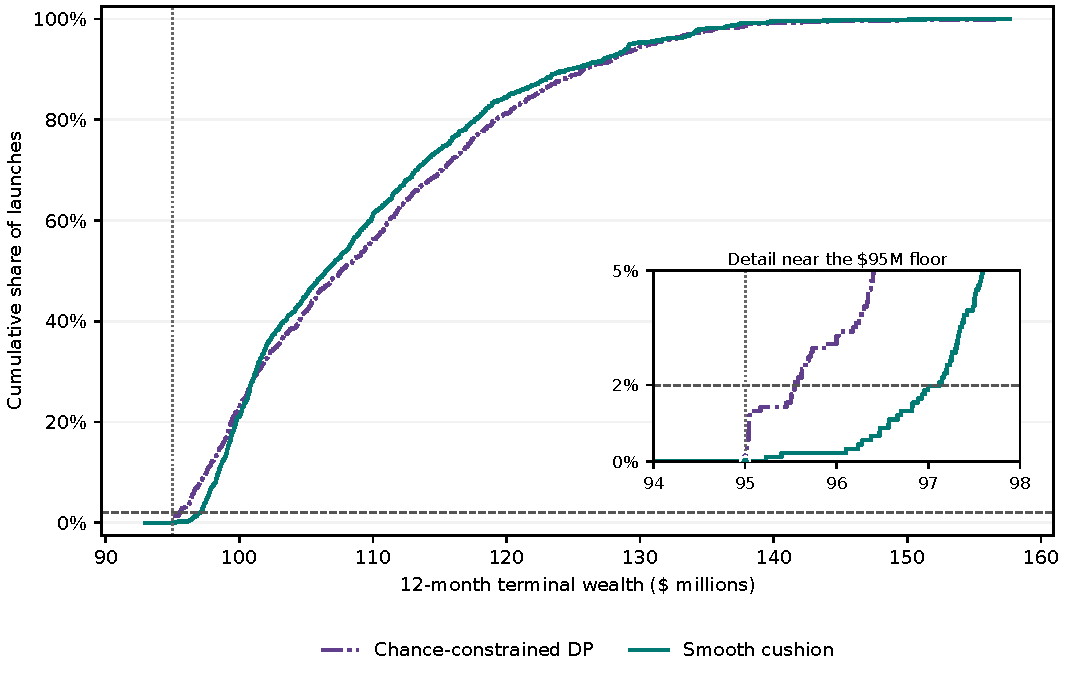
\includegraphics[width=0.87\textwidth]{figures/smooth-terminal-cdf.pdf}
 \caption{Terminal wealth for the chance-constrained DP and smooth cushion on the same 910 monthly launches as Figure~\ref{fig:ccdp-cdf}. The inset shows the share finishing at or below each wealth level from \$94 to \$98 million. Dots mark the share at \$95 million and the horizontal dashed line marks 2\%.}
 \label{fig:smooth-cdf}
\end{figure*}
